\documentclass{article}

\usepackage{times}
\usepackage[top=1in, bottom=1in, left=1in, right=1in]{geometry}
\usepackage{graphicx}
\usepackage{float}

\floatstyle{ruled}
\newfloat{program}{thp}{lop}
\floatname{program}{Program}

\begin{document}

\author{Joshua Ashby\\
\\
        With the help of:\\
        Maurice Ashby\\
\\
        Linux And Sci\\
                \texttt{http://joshashby.com}\\
		\texttt{joshuaashby@joshashby.com}}
\title{Project: Bouncing Off Bumpers}

  \begin{center}
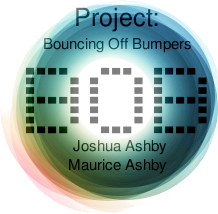
\includegraphics{boblogo}\\
\texttt{http://bob.joshashby.com}\\
\\
In Conjunction with:\\

\includegraphics{linuxandscilogo}\\
\texttt{http://joshashby.com}\\
  \end{center}

\maketitle

\newpage
\tableofcontents
\listoffigures
\newpage

\abstract{Bouncing off Bumpers, or BOB is a competition robot built by Joshua Ashby and his grandfather Maurice Ashby for the April 15th, 2009 Sparkfun Autonomous Vehicle Competition. It measures approximately 3 feet long by 2 feet wide by 2 feet tall; it weights approximately 50 pounds without the battery and electronics.
This paper will go into detail about the many systems involved in the build process of BOB, and provide insight into how many of these systems were designed, and the logic behind them (Please note that this paper is always going to be changing, and the data could easily change the day after the latest pubilishing).}\\
\section{Introduction and Background}
The electronics were designed by me (Joshua Ashby), and built by me along with the aid of my grandfather Maurice Ashby. As of December 1st, 2009 BOB now has the complete second generation electronics (which will be explained later on), and the plans and designs for the third generation electronics are under way.\\
The mechanics of the robot, which refers to the frame and body, the steering and related mechanisms, and the propulsion system were designed and built by us over a course of approximately 5 weeks.\\
\section{Frame\footnote{Please note, the frame was made to be cheap, and need little maintanince}%
}
\subsection{Shape, Design and Material}
In order to build the frame in both a time and cost effective way, we choose to reuse some old square steel tubing that measures and has a wall width of . Maurice had just enough laying around his shop to build a frame with. By using steel square tubing, and welding the joints, we were able to build a sturdy frame capable of carrying well over 100LBS.\\
The design of a three wheeled robot came after evaluating the cost of the wheels that would be used; to keep the cost down, only three wheels would be used. Because only three wheels would be used, the frame would have to be built in a fashion that did not promote tilting when the robot turns but still allow a large amount of room to build on top of. To accomplish this, an elongated pentagon design was created. The main drive wheel would be placed at the back of the robot in a triangle shaped portion of the frame, while the middle and front of the body would be a square shape, with two wheels in the front to steer with.\\
\subsection{Steering}
The steering for BOB was modeled after a car style steering system, where two wheels are connected via a rod which is in turn moved left or right to turn the wheels (Figure \ref{steering}).
\begin{figure}[htp]
  \begin{center}
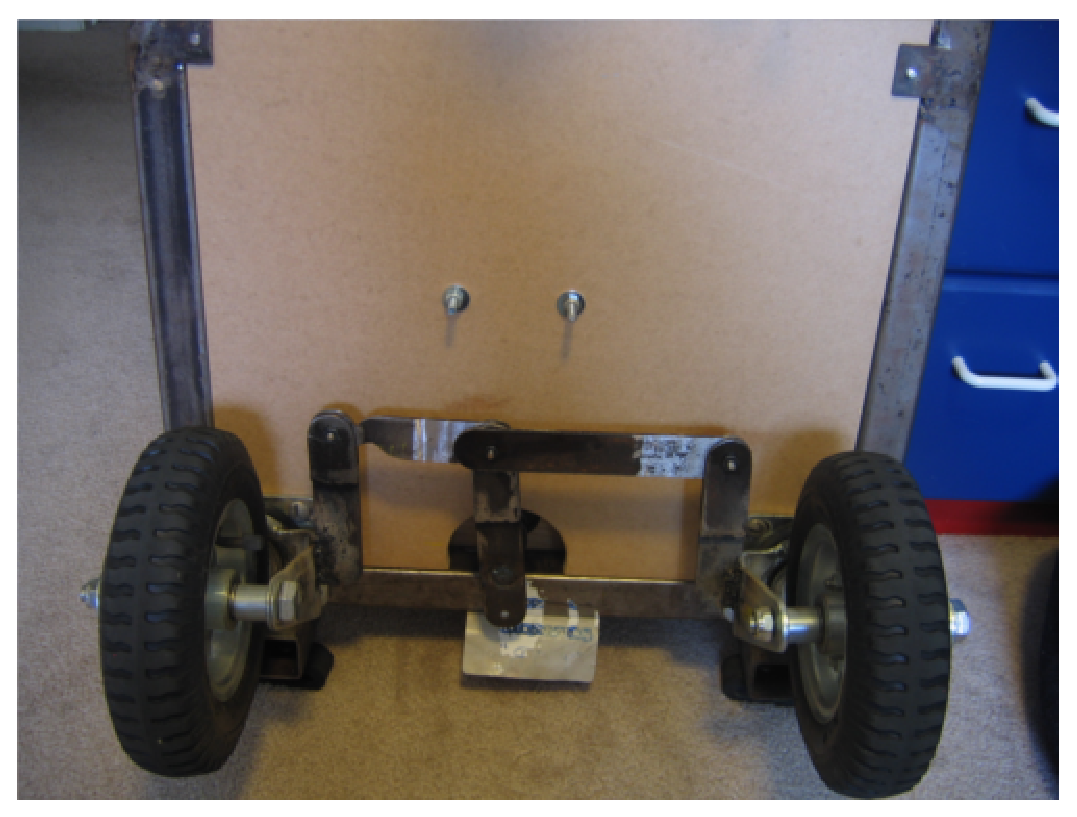
\includegraphics[scale=0.25]{steering}
  \end{center}
  \caption{Example of the steering build used}
\label{steering}
\end{figure}\\
The build of this was accomplished by using two pre-built wheel casters, and welding on strips of quarter inch thick steel. These strips are approximately 6 inches long, and at the end that is not welded to the caster wheels, there is a hole drilled. Then connecting the two wheels via these strips, is a second pair of steel strips that are hooked up to the steering motor.\\
The steering motor is a 9.6V 10A drill motor that has been mounted with a right angle drive. This allows the motor to lay flat with the robot frame and still be able to turn the steering rod (Figure \ref{steeringmotor}).
\begin{figure}[htp]
  \begin{center}
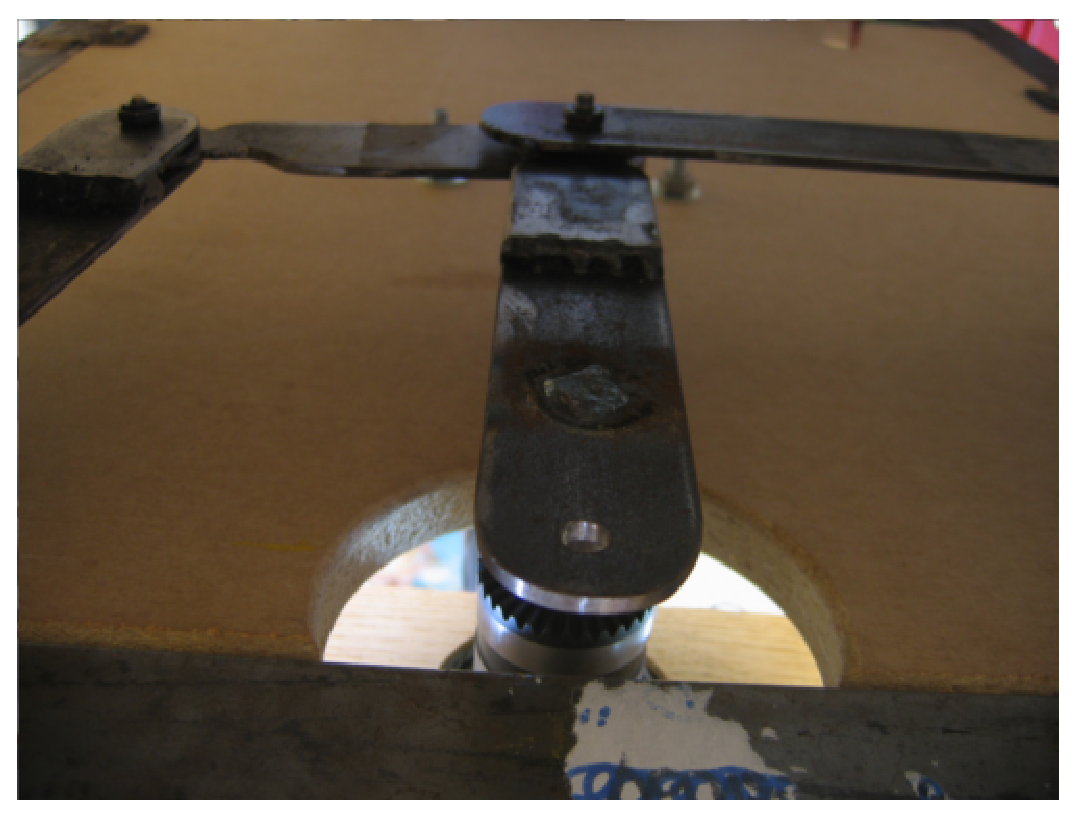
\includegraphics[scale=0.25]{steeringmotor}
  \end{center}
  \caption{Example of the steering motor}
\label{steeringmotor}
\end{figure}\\
One problem that was not foreseen while building the steering, is the ability to drive straight. Because the steering mechanism does not have a method of straighting it's self out, a new task is introduced to the electronics and programming. The accomplish this, generation 3 electronics may very well include 3 or more photo interrupts that are placed on the steering mechanism (Figure \ref{photogate}).
\begin{figure}[htp]
  \begin{center}
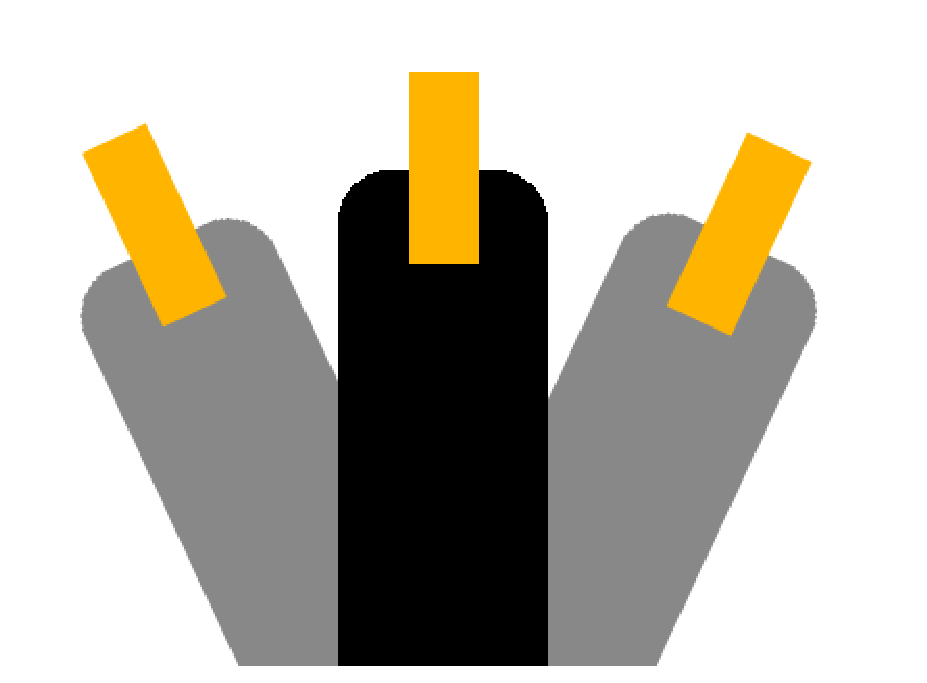
\includegraphics[scale=0.25]{photogate}
  \end{center}
  \caption{Example of the possible photogate layout}
\label{photogate}
\end{figure}\\
Using these photo interrupts would be either the Motor Node (see section Electronics) or a Sensor Node. This Node would then “listen” for one of these photo interrupts to change, at which point it would notify the Motor Node to turn the appropriate direction.\\
\subsection{Propulsion}
Transferring power from the drill motor to the back drive wheel was one of the greatest technical difficulties we encountered. We started off by testing the idea of a friction drive. This style of drive has the motor running parallel to the wheel, and the output shaft using friction to turn the wheel. This worked great going downhill, but as soon as the drive had a load to pull, such as on flat ground, or uphill, the drive would start to slip.\\
Our second attempt was based off of a bike, just instead of a chain drive, we decided to do a belt drive as Maurice had many of the needed parts. The motor was mounted perpendicular to the wheel, and had a small 1.25 inch radius belt pulley on it. The wheel then had a larger 4 inch radius diameter belt pulley on it. The two pulleys were connected via 8 inch diameter cogged belt. The axle for the motor is a milled axle that is supported by a bearing block at one end. The other end is tapered down to allow it to fit in the motor chuck. This also allows the motor to be disconnected from the axle, allowing the robot to be moved around with out power to the motor. (Figure \ref{reardrive}).
\begin{figure}[htp]
  \begin{center}
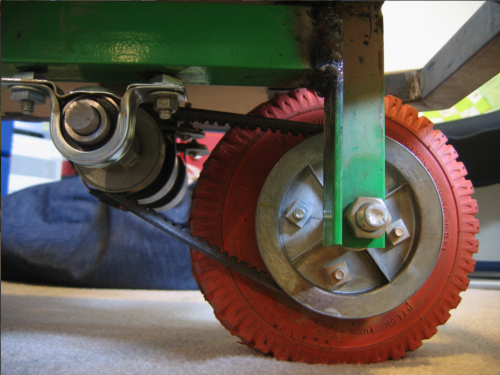
\includegraphics[scale=0.25]{reardrive}
  \end{center}
  \caption{Example of the drive system used}
\label{reardrive}
\end{figure}\\
This drive system worked perfectly both downhill and uphill, and as a result it is the drive system currently used. The motor is the same as the steering motor, a recycled drill motor that is rated at 9.6V and 10A.\\
\section{Electronics}
\subsection{Introduction}
The electronics have always been a troublesome matter for this project, and as this is being typed, the electronics still are providing issues that most of the time carry a re-design of the boards. The simplest task, providing power to the "Nodes" is the simplest and by far least bug prone of all the boards. The power is supplied from a small 12V motorcycle lead acid battery, which is connected to the motor rails, and the power distribution rails. The power distribution rails connect to the power node. This node takes the twelve volts, and regulates it down to five volts for the micro-controllers.\\
The motors, which draw ~10A, must have easy to use, and cheap to build motor controllers, along with the ability to easily replace a part while the robot is not in the Lab. This means the motor controllers can not be store bought, as all of the quality controllers that we can find are not only expensive, but also do not have common, easy to find parts. Instead to replace a part, the whole controller must be replaced most the time.\\
Generation 1 electronics consisted of one micro-controller, and one and a half motor controllers. These electronics shorted out at the 2009 Sparkfun AVC competition, and as a result will only be used as both a comparison, and as a resource for what not to do on future generations.\\
\subsection{Node Networking}
Generation 2 electronics allow for more than one micro-controller to be on the robot at one time via a communications protocol commonly called I2C. By using I2C we can add up to 255 “Nodes” to the robot, which can then allow us to hand out different tasks as needed, evening the work load out.\\
The addressing for this network is provided through a square of 4 header pins which are connected to digital input/output pins on each Node. By using jumpers to short out different combinations in these headers, currently 6 unique addresses can be generated. This allows for the Nodes to be removed, and added without having to change the address in software.\\
\subsection{Main Node}
The Main Node, or also what we call the Master Node is just as it's title calls it, the Master Node in the network. This Node is the gateway to the robot from a computer, it is the only Node equipped with USB serial communication permanently, and in the future, plans are made to have this Node equipped with wireless communication such as from an xBee module.\\
\subsection{Sensor Node\footnote{This Node is currently tied in with the Main Node on generation 2 electronics}}
The Sensor Node is responsible for gathering, and processing all of the data from various sensors. At the moment it is only in charge of the two forward ultrasounds, which it will read the values from, then determine if the Motor Node should turn left or right, or reverse.\\
\subsection{Motor Node}
As stated above, the use of store bought motor controllers is out of the question for use on BOB. They tend to be expensive, and typically must have the whole unit replaced if something burns out. Because of this, the motor controllers have been hand designed by us.\\
The first version, which is the version that was used during the 2009 Sparkfun AVC competition, was designed to be very simple, and yet still provide the power that was needed for the motors. It consisted of a TIP125 PNP transistor driving a pair of paralleled IRF540N n-channel MOSFETs. At the time of their designing and building, we both were very new to MOSFETs (which they continue to be fairly new to even after a year of using them) and as a result the knowledge of how to hook the MOSFETs up, and the voltage required to drive them was unknown. This caused many problems, such as the MOSFETs not having enough voltage and amperes for them to fully open up. This caused them to over heat, and also caused a massive power spike somewhere along the lines that burnt out the MOSFETs and transistor.\\
The new generation 2 motor controllers are designed to avoid these problems, along with begin to merge into a modular system as talked about in section Electronics: Introduction. These new motor controllers are now called the Motor Nodes, and include the two motor controllers, and the micro-controller that controls the controllers. The micro-controller for generation 2 electronics is an Atmega328. As talked about in section Electronics: II. Node Networking, this Atmega communicates with other Nodes, such as the Sensor or Main Node to receive commands about what actions it should take, such as whether or not to turn or go backwards.\\
Connecting the MOSFETs in a way that could provide 10A safely was a bit difficult, but the system currently used is a "block and tackle" style. The MOSFETs and diodes have short 12g wires soldered to their pins, with spade crimp connectors on the other end. The gates of the MOSFETs have female header crimp connectors instead to connect to the controller board. The spade connectors connect to a  terminal block, which is rated for 20A. This combinations allows for multiple MOSFETs and diodes to be connected to the same motor (Figure \ref{blockandtackle}).
\begin{figure}[htp]
  \begin{center}
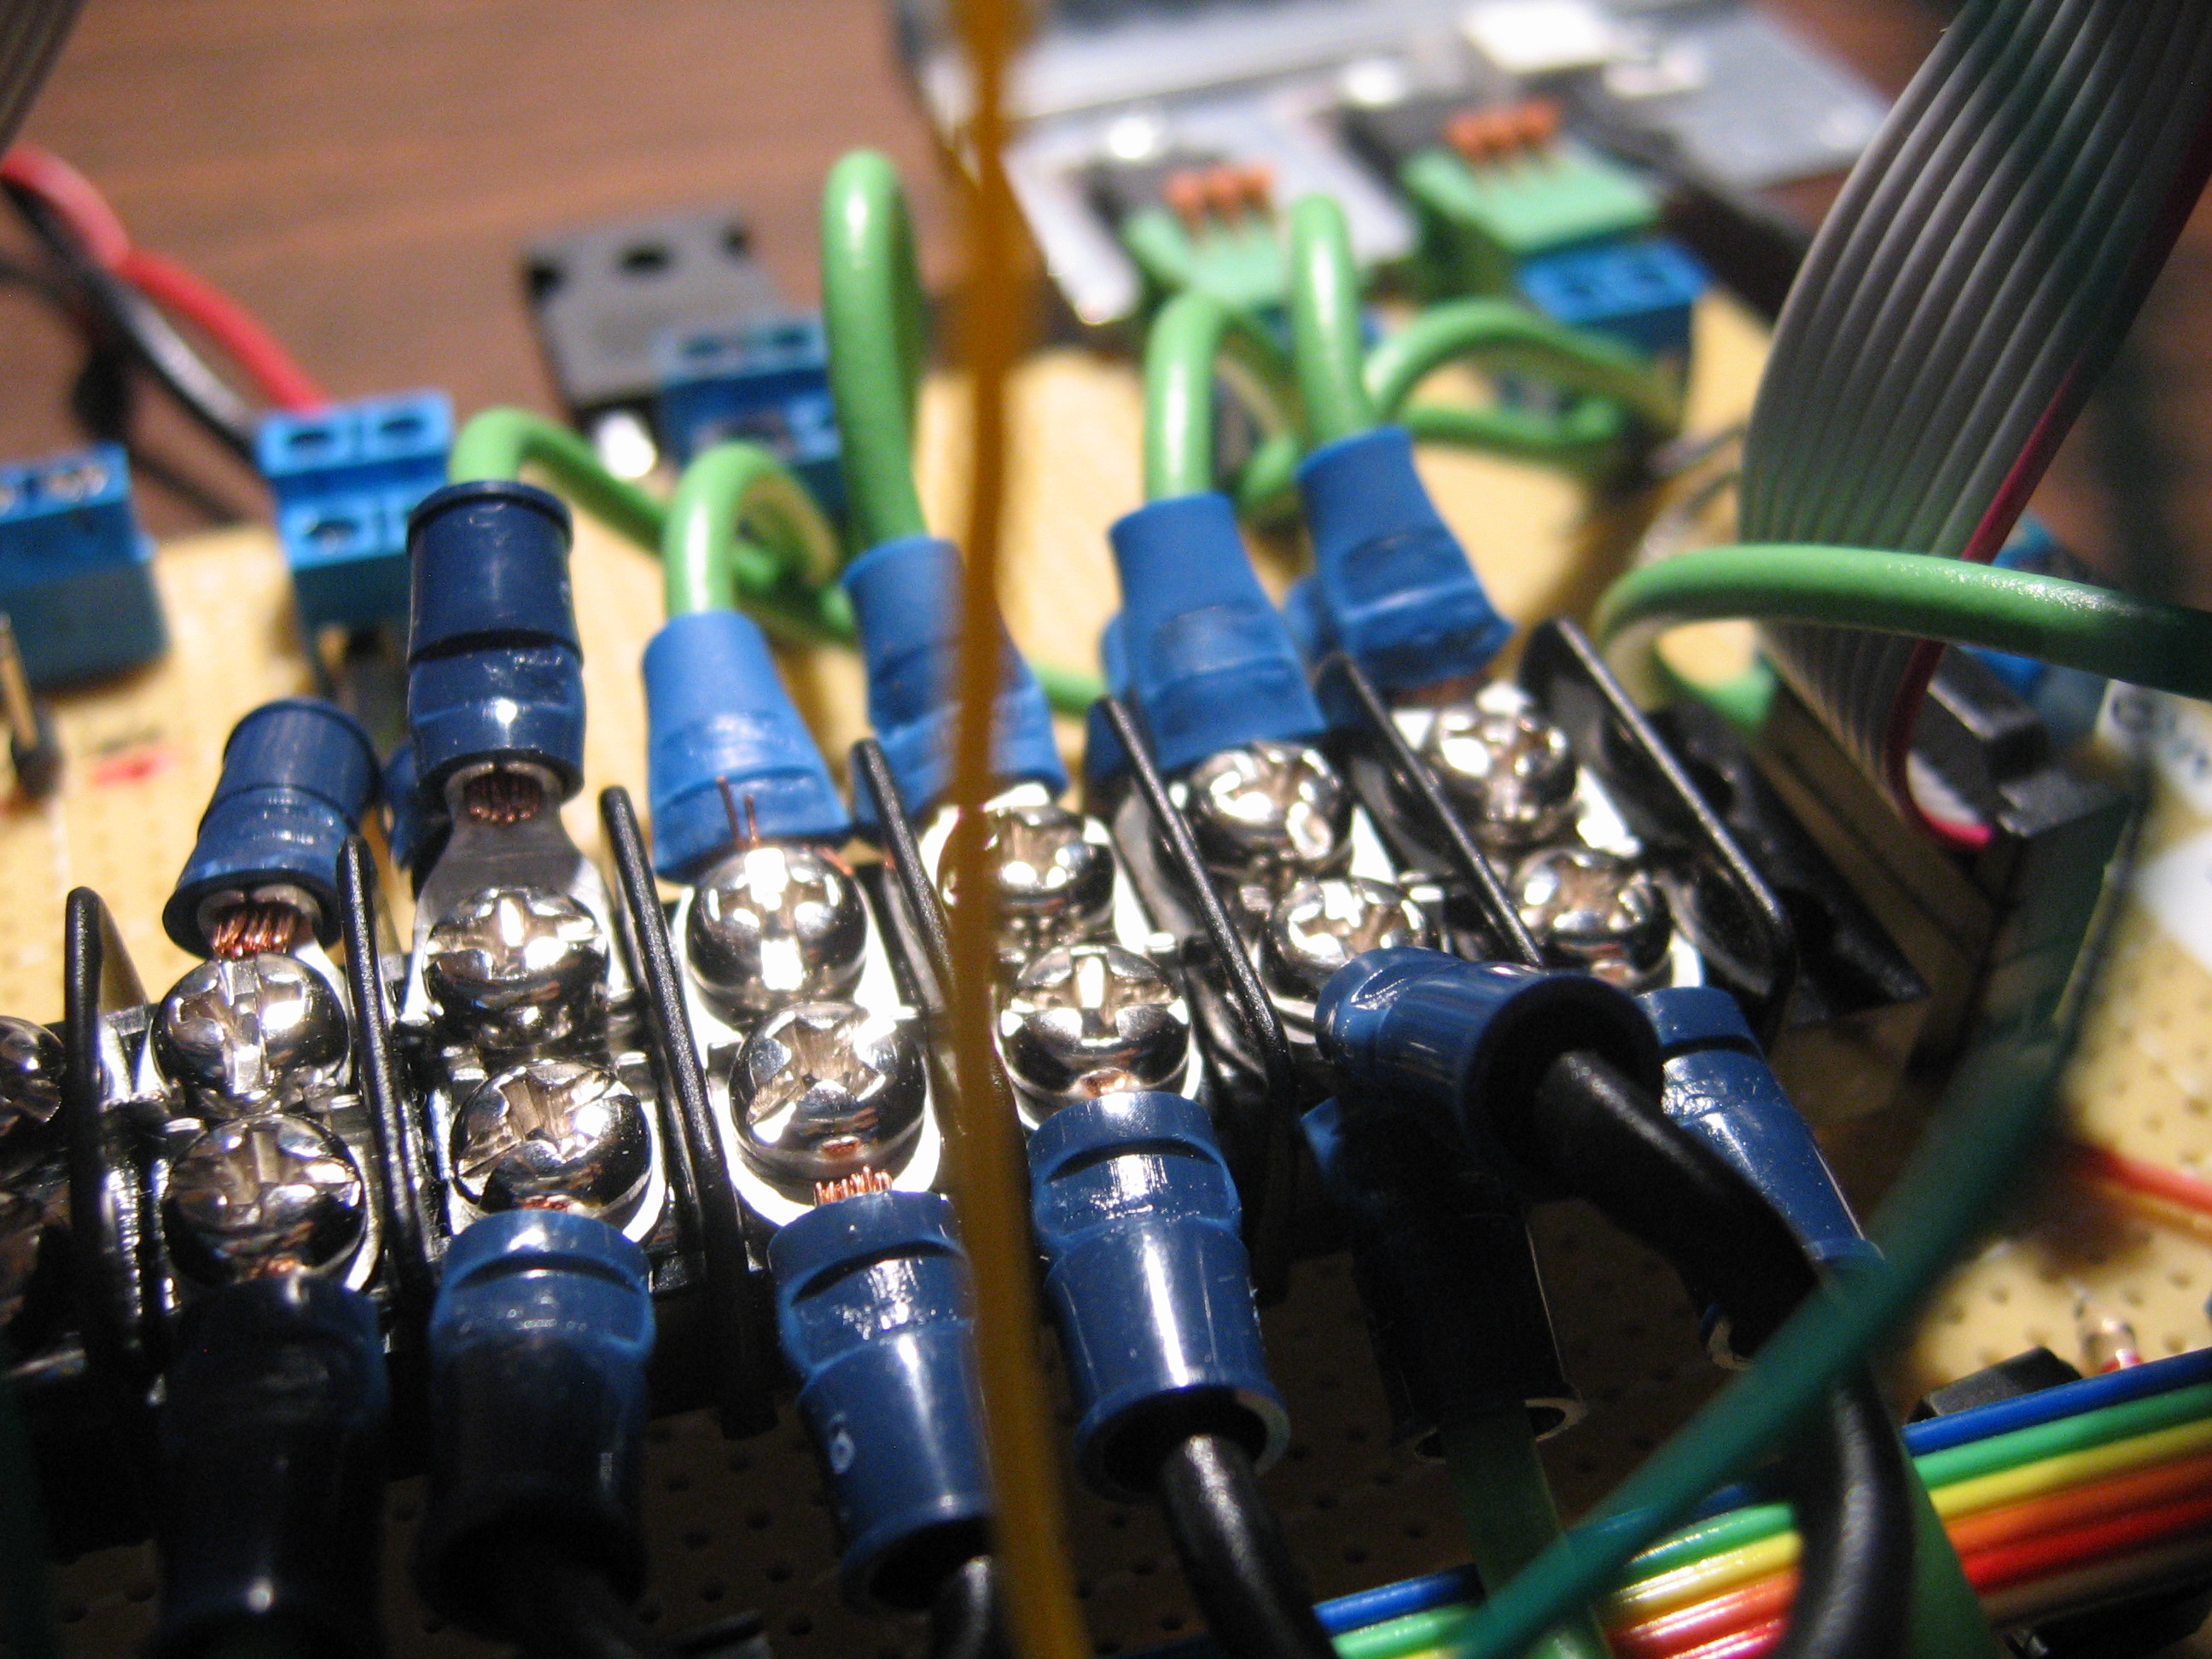
\includegraphics[scale=0.05]{blockandtackle}
  \end{center}
  \caption{Example of the Block and Tackle Style of Build used for the MOSFETs}
\label{blockandtackle}
\end{figure}\\
\subsection{Power Node}
The Power Node, as of generation 2 electronics is simply a “dead” Node as one might call it. It has no intelligence, instead it's only function for generation 2 is to regulate and distribute 5V to all the boards. It does this via Molex connectors off of old ATX power supplies from computers.\\
\section{Software}
\subsection{Robot side}
The robot side of the software stack is written in C, with the addition of the Arduino\footnote{Arduino - http://www.arduino.cc/} libraries. By using the Arduino libraries, fast prototyping of a new Node can be accomplished with out massive amounts of code. Also the understandability of the code is increased.\\
\subsection{Library}
To allow for quick prototyping of new Nodes, a basic library containing all of the functions used by every Node was written. In this library there is a function that figures out the address of the Node, then sets that address as the I2C address. This library also includes functions to turn on and off different pins on other micro-controllers, along with set the speed, direction and turning direction via I2C. Finally the library also includes at the moment functions to set the speed, direction and which way the robot is turning for use on the Motor Node.
The address is found with simple logic, by turning on the 1st pin, then reading the 2nd and 3rd pins, then turning off the 1st pin the micro-controller can figure out if pins 1 and 2 are shorted out, or if 1 and 3 are shorted out. Then, depending on which of those pins have been shorted out, the micro-controller turns on the 4th pin, and reads from either the 2nd or 3rd again, depending on which pin was shorted to pin 1 (Page \pageref{address}).\\
\subsection{Node Specific}
Most Nodes have individual functions that they do not share with other Nodes, such as the Motor Node, and the Sensor Node. These special functions must there for be written into the code for each Node.\\
\subsubsection{Main Node}
The Main Node, unlike the other nodes must have USB serial communications setup. This is because it is the only Node with USB capabilities. As a result, this Node's code must have a specific function for passing data back and forth from the I2C to the computer.\\
\subsubsection{Motor Node}
The Motor Node, unlike other Nodes must monitor the temperature of both motor controllers, and if the temperature rises beyond a set value, it must then turn off power to that controller. To do this, the hardware has thermistors hooked up to the analog input pins on the Atmega328.\\
\subsubsection{Sensor Node}
The Sensor Node is responsible for collecting the data from various sensors (just the ultrasounds right now) and processing that data to come up with an action.\\
\subsection{Computer Side}
Because the Main Node has USB capabilities, the whole robot is able to talk to the computer. As a result there is also computer software that is being developed to aid in the control, and monitoring of the robot. This software stack is being written in Python, but may include Perl or C in the future. The Pyserial module is used for the USB serial communication.\\
To be able to use the computer as a form of remote was a big advantage. To complete this, I wrote\footnote{In reality it was already mostly written for an previous robot} a GUI in Python that used the PyQt3 module for the GUI. This GUI simply had a "D pad" of sorts, 4 buttons arranged in a cross style layout which provided the options of going forward, backwards and turning in both directions (Program - \ref{dpad}).\\
\begin{program}
\begin{verbatim}
     | ^ | 
| < |     | > |
     | V |
\end{verbatim}
\caption{Layout of the D pad buttons}
\label{dpad}
\end{program}\\
The GUI also had space to provide feedback from the robot, but I have not gotten around to writing this part of the code\footnote{Due to many electrical related problems}. I have plans to re-write this GUI in the newer PyQt4, and add feedback, along with better joystick support as soon as the electrical problems are addressed. Until then software support for the computer side has stopped altogether.\\
\section{About the builders}
\subsection{Joshua Ashby}
\subsection{Maurice Ashby}
\begin{program}
\begin{verbatim}
void Robot::setAddress(int master)
{
  if (master == 1) {
     Wire.begin();
  }
  if (master == 0) {
     digitalWrite(_set1, HIGH);
     x = digitalRead(_set2);
     if (x == HIGH) {
        digitalWrite(_set4, HIGH);
        y = digitalRead(_set3);
        if (y == HIGH) {
           Wire.begin(5);
        }
        if (y == LOW) {
           Wire.begin(1);
        }
        digitalWrite(_set4, LOW);
     }
     if (x == LOW) {
        digitalWrite(_set1, LOW);
        digitalWrite(_set4, HIGH);
        x = digitalRead(_set3);
        if (x == HIGH) {
           Wire.begin(2);
        }
        digitalWrite(_set4, LOW);
     }
     x = digitalRead(_set3);
     if (x == HIGH) {
        digitalWrite(_set4, HIGH);
        y = digitalRead(_set2);
        if (y == HIGH) {
           Wire.begin(6);
        }
        if (y == LOW) {
           Wire.begin(3);
        }
        digitalWrite(_set4, LOW);
     }
     if (x == LOW) {
        digitalWrite(_set1, LOW);
        digitalWrite(_set4, HIGH);
        y = digitalRead(_set2);
        if (y == HIGH) {
           Wire.begin(4);
        }
        digitalWrite(_set4, LOW);
     }
  }
}
\end{verbatim}
\caption{Sample of the code used to set the I2C address}
\label{address}
\end{program}

%\cite{langley96}
%\footnote{}
%\emph{performance stage}

%\bibliographystyle{plain}
%\bibliographystyle{alpha}
%\bibliographystyle{unsrt}
%\bibliographystyle{abbrv}

%\bibliographystyle{IEEEtranS}
%\bibliographystyle{cj}

%\bibliography{bib}

\end{document}
